%%%%%%%%%%%%%%%%%%%%%%%%%%%%%%%%%%%%%%%%%%%%%%%%%%%%%%%%%%%%%%%%%%%%%%%%%%%%%%%%%%
\begin{frame}[fragile]\frametitle{}
\begin{center}
{\Large Plotting}
\end{center}
\end{frame}

%%%%%%%%%%%%%%%%%%%%%%%%%%%%%%%%%%%%%%%%%%%%%%%%%%%%%%%%%%%%%%%%%%%%%%%%%%%%%%%%%%%
\begin{frame}[fragile]\frametitle{matplotlib: publication quality plotting library}

\begin{itemize}
\item   \href{http://matplotlib.org/}{matplotlib} is a python 2D plotting
  library for quality figures
\item matplotlib can be used in python scripts, the python and
  ipython shell (ala MATLAB or Mathematica), web application
  servers, and six graphical user interface toolkits
    \item Tutorial: {\footnotesize\url{http://www.loria.fr/~rougier/teaching/matplotlib/}}
  \item Examples: {\footnotesize\url{http://matplotlib.org/1.2.1/gallery.html}}
\end{itemize}

\end{frame}

%%%%%%%%%%%%%%%%%%%%%%%%%%%%%%%%%%%%%%%%%%%%%%%%%%%%%%%%%%%%%%%%%%%%%%%%%%%%%%%%%%%
\begin{frame}[fragile]\frametitle{What is Matplotlib?}
    
    \begin{itemize}
        \item Matplotlib is a rendering API for 2D (and limited 3D) plotting
        \item \lstinline|matplotlib.pyplot| is a streamlined Matlab-like interface to Matplotlib
        \item \lstinline|pylab| is a bundle of NumPy, SciPy and Matplotlib.\\
        One often sees it invoked like this:
        \begin{lstlisting}
from pylab import *
        \end{lstlisting}
    \end{itemize}
\end{frame}

%%%%%%%%%%%%%%%%%%%%%%%%%%%%%%%%%%%%%%%%%%%%%%%%%%%%%%%%%%%%%%%%%%%%%%%%%%%%%%%%%%%
\begin{frame}[fragile]
    \frametitle{My First Plot}

    Plot $\sin x$ from $-2\pi$ to $2\pi$:
        \begin{lstlisting}
import numpy as np
import matplotlib.pyplot as plt

x = np.linspace(-2.*np.pi, 2.*np.pi, 100)
y = np.sin(x)

plt.plot(x, y)
plt.show()
        \end{lstlisting}
\begin{center}
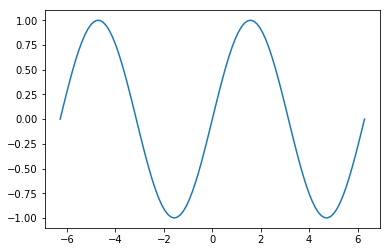
\includegraphics[width=0.5\linewidth,keepaspectratio]{44}
\end{center}
\end{frame}

%%%%%%%%%%%%%%%%%%%%%%%%%%%%%%%%%%%%%%%%%%%%%%%%%%%%%%%%%%%%%%%%%%%%%%%%%%%%%%%%%%%
\begin{frame}[fragile]\frametitle{Saving your Figure}

    Append this to the end of your script:
    \begin{lstlisting}
plt.savefig('myplot.pdf')
    \end{lstlisting}
    It usually figures out the file type from the extension.
    \\~\\
    To remove space around the plot, use:
    \begin{lstlisting}
plt.savefig('myplot.pdf', bbox_inches='tight')
    \end{lstlisting}

\end{frame}

%%%%%%%%%%%%%%%%%%%%%%%%%%%%%%%%%%%%%%%%%%%%%%%%%%%%%%%%%%%%%%%%%%%%%%%%%%%%%%%%%%%
\begin{frame}[fragile]\frametitle{Multiple Plots}

    Plot three sine curves with different phase shifts:
    $y_n = \sin(x + \phi_n)$
    \\~\\
    Call \lstinline|plot()| three times, then \lstinline|show()| the results
    \begin{lstlisting}
import numpy as np
import matplotlib.pyplot as plt

x = np.linspace(-2.*np.pi, 2.*np.pi, 100)
phase = np.arange(0., 2*np.pi, 2*np.pi/3.)

y_n = [np.sin(x + p) for p in phase]

for y in y_n:
    plt.plot(x, y)
plt.show()
    \end{lstlisting}
\begin{center}
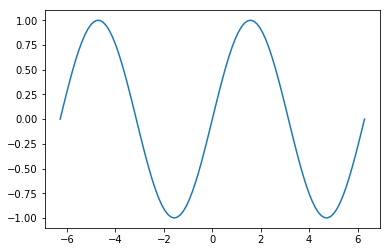
\includegraphics[width=0.25\linewidth,keepaspectratio]{46}
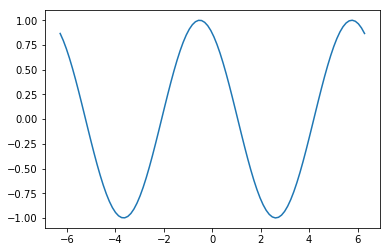
\includegraphics[width=0.25\linewidth,keepaspectratio]{46_1}
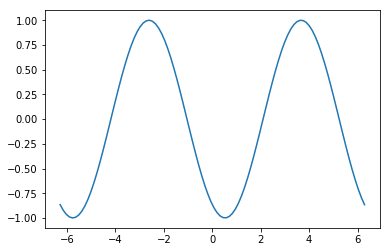
\includegraphics[width=0.25\linewidth,keepaspectratio]{46_2}
\end{center}
\end{frame}

%%%%%%%%%%%%%%%%%%%%%%%%%%%%%%%%%%%%%%%%%%%%%%%%%%%%%%%%%%%%%%%%%%%%%%%%%%%%%%%%%%%
\begin{frame}[fragile]\frametitle{Dots and Dashes}

    Stylise curves with dashes, shapes, and colours (like Matlab):
    \begin{lstlisting}
import numpy as np
import matplotlib.pyplot as plt

x = np.linspace(-2.*np.pi, 2.*np.pi, 50)
phase = np.arange(0., 2*np.pi, 2*np.pi/3.)

y_p = [np.sin(x + p) for p in phase]
style = ['r:', 'g--', 'py']

pdata = zip(y_p, style)
for y,s in pdata:
    plt.plot(x, y, s)
plt.show()
    \end{lstlisting}
\begin{center}
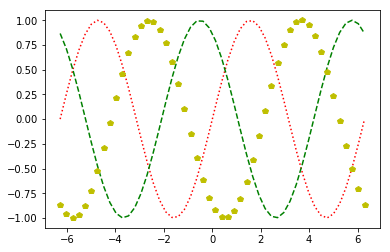
\includegraphics[width=0.25\linewidth,keepaspectratio]{47}
\end{center}
\end{frame}

%%%%%%%%%%%%%%%%%%%%%%%%%%%%%%%%%%%%%%%%%%%%%%%%%%%%%%%%%%%%%%%%%%%%%%%%%%%%%%%%%%%
\begin{frame}[fragile]
    \frametitle{Axis Labels}

    Labeling axes is similar to Matlab:
    \begin{lstlisting}
import numpy as np
import matplotlib.pyplot as plt

x = np.linspace(-2.*np.pi, 2.*np.pi, 100)
phase = np.arange(0., 2*np.pi, 2*np.pi/3.)
y_n = [np.sin(x + p) for p in phase]

for y in y_n:
    plt.plot(x, y)

plt.title('Three-phase plots')
plt.xlabel('x')
plt.ylabel('y')
plt.show()
    \end{lstlisting}
\begin{center}
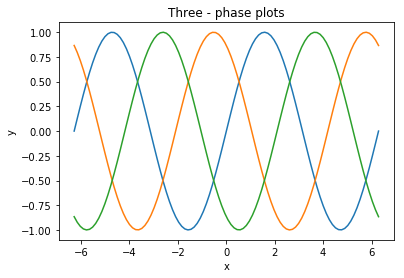
\includegraphics[width=0.25\linewidth,keepaspectratio]{48}
\end{center}
\end{frame}
%%%%%%%%%%%%%%%%%%%%%%%%%%%%%%%%%%%%%%%%%%%%%%%%%%%%%%%%%%%%%%%%%%%%%%%%%%%%%%%%%%%
\begin{frame}[fragile]\frametitle{Legends}

    Include a legend in your plot
    \begin{lstlisting}
import numpy as np
import matplotlib.pyplot as plt

x = np.linspace(-2.*np.pi, 2.*np.pi, 100)
phase = np.arange(0., 2*np.pi, 2*np.pi/3.)
y_n = [np.sin(x + p) for p in phase]

for y in y_n:
    plt.plot(x, y)

legend_text = ['$\phi$ = %.2f' % p
                            for p in phase]
plt.legend(legend_text)
plt.show()
    \end{lstlisting}
\begin{center}
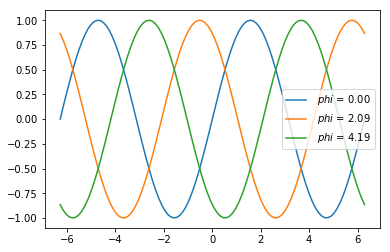
\includegraphics[width=0.25\linewidth,keepaspectratio]{49}
\end{center}
\end{frame}

%%%%%%%%%%%%%%%%%%%%%%%%%%%%%%%%%%%%%%%%%%%%%%%%%%%%%%%%%%%%%%%%%%%%%%%%%%%%%%%%%%%
\begin{frame}[fragile]\frametitle{Contour Plots}

    Plot contours on range $[-2,2]\times[-2,2]$ for the function:
    \[ z(x, y) = \left(x - \frac{1}{2}\right) e^{-\sqrt(x^2 + y^2)} \]
    \begin{lstlisting}
import numpy as np
import matplotlib.pyplot as plt
x_ax = np.linspace(-2., 2., 100)
y_ax = np.linspace(-2., 2., 100)
x, y = np.meshgrid(x_ax, y_ax)
z = (x - 0.5)*np.exp(-np.sqrt(x**2 + y**2))
plt.contour(x, y, z, 25)
plt.show()
    \end{lstlisting}
\begin{center}
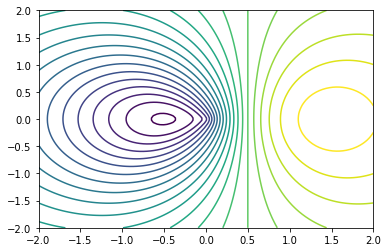
\includegraphics[width=0.25\linewidth,keepaspectratio]{50}
\end{center}
\end{frame}

%%%%%%%%%%%%%%%%%%%%%%%%%%%%%%%%%%%%%%%%%%%%%%%%%%%%%%%%%%%%%%%%%%%%%%%%%%%%%%%%%%%
\begin{frame}[fragile]
    \frametitle{Image Plots}

    \lstinline|imshow| plots pixel fields (\lstinline|pcolor| is very slow)
    \begin{lstlisting}
import numpy as np
import matplotlib.pyplot as plt
x_ax = np.linspace(-2., 2., 100)
y_ax = np.linspace(-2., 2., 100)
x, y = np.meshgrid(x_ax, y_ax)
z = (x-0.5) * np.exp(-np.sqrt(x**2 + y**2))
z_ext = (x_ax[0], x_ax[-1], y_ax[0], y_ax[-1])
plt.imshow(z, origin='lower', extent=z_ext)
plt.show()
    \end{lstlisting}
\begin{center}
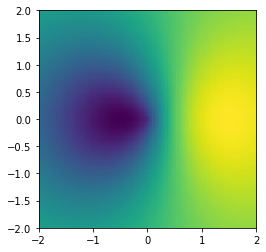
\includegraphics[width=0.25\linewidth,keepaspectratio]{51}
\end{center}
\end{frame}

%%%%%%%%%%%%%%%%%%%%%%%%%%%%%%%%%%%%%%%%%%%%%%%%%%%%%%%%%%%%%%%%%%%%%%%%%%%%%%%%%%%
\begin{frame}[fragile]
    \frametitle{Object-Oriented Matplotlib}
    As your plots become more complex, you may need to start using object-oriented matplotlib
    \begin{lstlisting}
import numpy as np
import matplotlib.pyplot as plt

x = np.linspace(-2.*np.pi, 2.*np.pi, 100)
y = np.sin(x)

fig = plt.figure()
ax = fig.add_subplot(1,1,1)
line = ax.plot(x, y)
ax.set_xlim([-2*np.pi,2*np.pi])

plt.show()
    \end{lstlisting}
\begin{center}
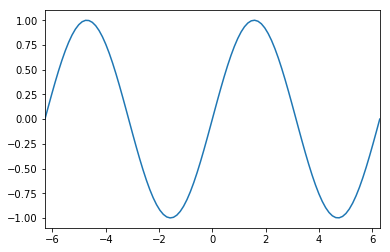
\includegraphics[width=0.25\linewidth,keepaspectratio]{52}
\end{center}
\end{frame}

%%%%%%%%%%%%%%%%%%%%%%%%%%%%%%%%%%%%%%%%%%%%%%%%%%%%%%%%%%%%%%%%%%%%%%%%%%%%%%%%%%%
\begin{frame}[fragile]\frametitle{Subplots}

    Put two plots on the same figure:
    \begin{lstlisting}
import numpy as np
import matplotlib.pyplot as plt

x = np.linspace(-2.*np.pi, 2.*np.pi, 100)
y1 = np.sin(x)
y2 = np.cos(x)

fig, (ax1, ax2) = plt.subplots(nrows=2,
                               ncols=1)
ax1.plot(x, y1)
ax2.plot(x, y2)

plt.show()
    \end{lstlisting}
\begin{center}
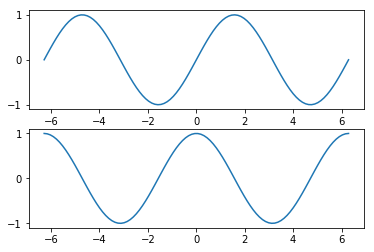
\includegraphics[width=0.25\linewidth,keepaspectratio]{53}
\end{center}
\end{frame}

%%%%%%%%%%%%%%%%%%%%%%%%%%%%%%%%%%%%%%%%%%%%%%%%%%%%%%%%%%%%%%%%%%%%%%%%%%%%%%%%%%%
\begin{frame}[fragile]\frametitle{Basemap: Earth Grid Plotting}

    Basemap provides tools for plotting on several geographic grids.
\end{frame}

%%%%%%%%%%%%%%%%%%%%%%%%%%%%%%%%%%%%%%%%%%%%%%%%%%%%%%%%%%%%%%%%%%%%%%%%%%%%%%%%%%%
\begin{frame}[fragile]\frametitle{Orthographic Grids}
    \begin{lstlisting}
from mpl_toolkits.basemap import Basemap
import numpy as np
import matplotlib.pyplot as plt

m = Basemap(projection='ortho',lon_0=-105,
            lat_0=40,resolution='l')
m.drawcoastlines()
m.fillcontinents(color='coral',
                 lake_color='aqua')
m.drawparallels(np.arange(-90.,120.,30.))
m.drawmeridians(np.arange(0.,420.,60.))
m.drawmapboundary(fill_color='aqua')
plt.show()
    \end{lstlisting}
\end{frame}

%%%%%%%%%%%%%%%%%%%%%%%%%%%%%%%%%%%%%%%%%%%%%%%%%%%%%%%%%%%%%%%%%%%%%%%%%%%%%%%%%%%
\begin{frame}[fragile]\frametitle{Mercator Grids}
    \begin{lstlisting}
from mpl_toolkits.basemap import Basemap
import numpy as np
import matplotlib.pyplot as plt
m = Basemap(projection='merc',llcrnrlat=-80,
            urcrnrlat=80, llcrnrlon=-180,
            urcrnrlon=180,lat_ts=20,
            resolution='c')
m.drawcoastlines()
m.fillcontinents(color='coral',
                 lake_color='aqua')
m.drawparallels(np.arange(-90.,91.,30.))
m.drawmeridians(np.arange(-180.,181.,60.))
m.drawmapboundary(fill_color='aqua')
plt.show()
    \end{lstlisting}
\begin{center}
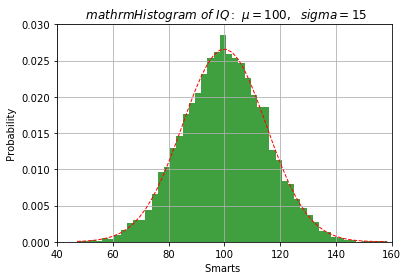
\includegraphics[width=0.25\linewidth,keepaspectratio]{57}
\end{center}
\end{frame}


%%%%%%%%%%%%%%%%%%%%%%%%%%%%%%%%%%%%%%%%%%%%%%%%%%%%%%%%%%%%%%%%%%%%%%%%%%%%%%%%%%%
\begin{frame}[fragile]\frametitle{\emph{Vectors} and \emph{Complex Numbers}}

\begin{lstlisting}
import numpy as np
import matplotlib.mlab as mlab
import matplotlib.pyplot as plt

mu, sigma = 100, 15
x = mu + sigma*np.random.randn(10000)
# the histogram of the data
n, bins, patches = plt.hist(x, 50, normed=1, facecolor='green', 
alpha=0.75)
# add a 'best fit' line
y = mlab.normpdf( bins, mu, sigma)
l = plt.plot(bins, y, 'r--', linewidth=1)
plt.xlabel('Smarts')
plt.ylabel('Probability')
plt.title(r'$\mathrm{Histogram\ of\ IQ:}\ \mu=100,\ \sigma=15$')
plt.axis([40, 160, 0, 0.03])
plt.grid(True)
plt.show()
\end{lstlisting}

\end{frame}

%%%%%%%%%%%%%%%%%%%%%%%%%%%%%%%%%%%%%%%%%%%%%%%%%%%%%%%%%%%%%%%%%%%%%%%%%%%%%%%%%%%
\begin{frame}[fragile]\frametitle{\emph{Vectors} and \emph{Complex Numbers}}
\begin{center}
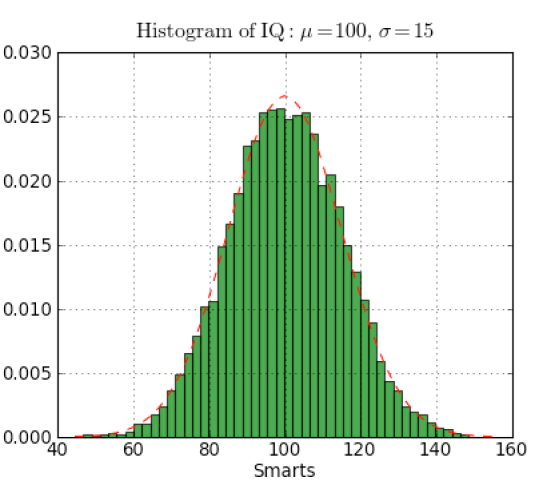
\includegraphics[width=0.75\linewidth,keepaspectratio]{matplotlibhist}
\end{center}
\end{frame}